\documentclass[a4paper,11pt]{article}
\usepackage{color}
\usepackage{graphicx}
\usepackage{subcaption}
\usepackage{amsmath}

\graphicspath{ {images/} }
\begin{document}
\title{\color{red}CARNEGIE MELLON UNIVERSITY\\
APPLIED STOCHASTIC PROCESSES  (COURSE 18-751)\\
HOMEWORK 2}
\author{Daniel Marew}
\date{\today}
\clearpage\maketitle

\thispagestyle{empty}
\newpage
I collaborated with :\\
\hspace*{6cm}
Nebyou Yismaw\\
\hspace*{6cm}
Daniel    Nkemelu\\
\hspace*{6cm}
Agatha Niwomugizi
\thispagestyle{empty}
\newpage


\newpage
\clearpage
\setcounter{page}{1}
\section*{Q.1\quad Compute the expected discounted future reward($\gamma (i)$)}
we can compute the expected discounted future reward by using the following formula
\begin{equation}
\gamma(i) = h(i) + \beta \sum_{j}P(i,j)\gamma(j)
\end{equation}•
where $\beta$ is the discount factor and $h(i)$ is the reward on state $i$.
\begin{equation}\label{eq:2}
\gamma(A) = 0 +  0.8*(0.5*\gamma(B)+0.5*\gamma(D))
\end{equation}•
\begin{eqnarray}
\gamma(B) = 0 +  0.8*\gamma(C)\\
\gamma(C) = 0 +  0.8*\gamma(A)\\
\gamma(D) = 1 +  0.8*(\frac{1}{3}*\gamma(B)+\frac{1}{3}*\gamma(E)+\frac{1}{3}*\gamma(A))\\
\gamma(E) = 2 +  0.8*(0.5*\gamma(B)+0.5*\gamma(C))
\end{eqnarray}•
Lets write all of them in terms of  $\gamma(A)$\\\\
\begin{eqnarray}
\gamma(A) = \gamma(A)\\
\gamma(B) = 0.64*\gamma(A)\\
\gamma(C) = 0.8*\gamma(A)\\
\gamma(D) = 1.5333+0.5909*\gamma(A)\\
\gamma(E) = 2+0.576*\gamma(A)
\end{eqnarray}•
writing eqn (\ref{eq:2}) interms of $\gamma(A)$s we get \\
\begin{eqnarray}
\gamma(A) = 0.64\gamma(A) + 0.4*0.5909*\gamma(A) + 0.4*1.5333\\
0.50764*\gamma(A) = 0.4*1.5333
\end{eqnarray}
so $\gamma(A)=1.2082$ ,$\gamma(A)=1.2082$,\quad $\gamma(B)=0.64*\gamma(A)=0.7732$,\\ \quad$\gamma(C)=0.8*\gamma(A)=0.9666$,\quad$\gamma(D)=1.5333+0.5909*\gamma(A)=2.2472$,\quad$\gamma(E)=2+0.576*\gamma(A)=2.6959$\\\\
Ans.\\
$\gamma(A)=1.2082$,\quad $\gamma(B))=0.7732$,\quad $\gamma(C))=0.9666$,\quad $\gamma(D))=2.2472$,\quad $\gamma(E))=2.6959$
\newpage
\section*{Q.2\quad Prove the following}

\begin{equation}
\bigcap\limits_{i=1}^{\infty}E_{i} \subset\Bigg(\bigcap\limits_{i=1}^{\infty}E_{i}^c\Bigg)^c 
\end{equation}•\\
soln.\\
We can rewrite the RHS as (\ref{eq:3}) using De Morgan's law\\
\begin{equation}\label{eq:3}
\Bigg(\bigcap\limits_{i=1}^{\infty}E_{i}^c\Bigg)^c = \bigcup\limits_{i=1}^{\infty}E_{i} 
\end{equation}•\\
To prove that the LHS is a subset of RHS we can show that any arbitrary element of LHS is also an element if the RHS.\\
lets say $e_{i}$ is an arbitrary element of LHS,  i.e $e_{i} \in \bigcap\limits_{i=1}^{\infty}E_{i} $ .This implies 
$e_{i}$ is an element of any set $E_{i}$ in the intersection. Since all the elements of arbitrary set $E_{i}$ are also  elements of the union of the sets, $e_{i} \in \bigcup\limits_{i=1}^{\infty}E_{i}$ .\\
Hence LHS is a subset of RHS. i.e $\bigcap\limits_{i=1}^{\infty}E_{i} \subset  \bigcup\limits_{i=1}^{\infty}E_{i} $
which is the same as saying,\\
\begin{equation}
\bigcap\limits_{i=1}^{\infty}E_{i} \subset\Bigg(\bigcap\limits_{i=1}^{\infty}E_{i}^c\Bigg)^c 
\end{equation}•\\
 Can the left and right side ever be equal?\\
 \textbf{YES}. When for example $E_{1}=E_{2}=E_{3}...=E_{i}=......$ , that is when all the $E_{i}$ s are the same.
 The intersection and union of those sets would be the same as  $E_{i}$.
\newpage
\section*{Q.3\quad }
%\mathcal{F}
\subsection*{(a) Show that the following statements are consistant with the three axioms of probability}
The three axioms of probability are :\\
(1)$P(A) \ge 0$ for all $A \subset S$ \\
(2)$P(S) = 1$\\
(3) if $A \cap B = \o$, then $P(A \cup B = P(A)+P(B)$  \\\\
Assigning $P[\{1\}]=1$, $P[\{2\}]=1$ , $P[\{1,2\}]=2$ is consistant with the first axiom because all the elements of $\mathcal{F}$ have $P \ge 0$, we can also assign $P(S) = P(\{1,2,3,4,5,6\}) = 1$ so it satisfies the second axiom.
When it comes to the third axiom, the only elements of $\mathcal{F}$ that are pair wise disjoint are \{1\} and \{2\}.\\\\
 $P(\{1\}\cup \{2\})=P(\{1,2\}) = 2 = P(\{1\}) + P(\{2\})$ hence it is also consitstant with third axiom.\\
 Therefore, $P[\{1\}]=1$, $P[\{2\}]=1$ , $P[\{1,2\}]=2$ is consistant with the three axioms of probability.

\subsection*{(b)}

\subsubsection*{Is $\mathcal{F}$ a sigma field?}
\textbf{NO}.\\
To be a sigma field $\mathcal{F}$ has to be closed under complementation.We can clearly see that $\mathcal{F}$ doesn't satisfy this property.$\{1\}^c$,$\{2\}^c$ and $\{1,2\}^c$ are all missing. \\
\subsubsection*{Minimum number of additional events required to make  $\mathcal{F}$ a sigma field.}
\textbf{3}.\\
we need to add $\{1\}^c$ which is $\{2,3,4,5,6\}$ ,$\{2\}^c$ which is $\{1,3,4,5,6\}$ and finally $\{1,2\}^c$ which is $\{3,4,5,6\}$ .\\
\begin{equation}\label{eq:new_f}
\mathcal{F} = \{ \o , \{1\},\{2\},\{1,2\},\{3,4,5,6\},\{1,3,4,5,6\},\{2,3,4,5,6\},\{1,2,3,4,5,6\}\}
\end{equation}•
\subsubsection*{Show that (a) is not true}
for $\mathcal{F}$ in (\ref{eq:new_f}) if we assign  $P[\{1\}]=1$, $P[\{2\}]=1$ , $P[\{1,2\}]=2$\\
$\implies P(\{1,2\} \cup \{3,4,5,6\})= P(\{1,2,3,4,5,6\})=P(S)$ \\
lets assume  it is consistant with the second and third axiom,\\ that means $P(S)= P(\{1,2\})+P(\{3,4,5,6\})=1$\\
 $$P(\{1,2\})+P(\{3,4,5,6\}) = 1$$
 $$2+ P(\{3,4,5,6\}) = 1 $$
 $$ P(\{3,4,5,6\}) = -1 $$
 i.e $P(\{3,4,5,6\}) \le 0$, thus violating the first axiom of probability.\\
 So $P[\{1\}]=1$, $P[\{2\}]=1$ and $P[\{1,2\}]=2$ will not be consistant with the  axioms of probability if $\mathcal{F}$ is a sigma field.
 
\newpage
\section*{Q4}
\subsection*{(a) No Kings}
We have 48 cards that are not King cards, hence we can select four cards that are not king cards in ${48 \choose 4} = 194580 $  different ways. \\\\
Ans. 194580
\subsection*{(b) 2 Kings and 2 Queens}
We have four kings so we can select two of them in ${ 4 \choose 2}$ ways similarly we can draw two Queens in  ${ 4 \choose 2}$ ways. Hence we can draw two Kings and two Queens in ${ 4 \choose 2}*{ 4 \choose 2}=36$ ways.\\\\
Ans. 36

\subsection*{(c) Number of Possible combinations of $(n_h,n_d,n_s,n_c)$}

Since we are drawing 4 cards 
\begin{equation}\label{eq:nr}
n_h+n_d+n_s+n_c = 4
\end{equation}•
The solutions for eqn(\ref{eq:nr}) make up the possible combinations of $(n_h,n_d,n_s,n_c)$.
the number of possible  solutions for eqn(\ref{eq:nr}) is given by $${{n+r-1} \choose r}$$
where $n$ is the number of possible outcomes(hearts,diamonds,spades and clubs) in this case 4 and $r$ is the number of times the experiment is conducted in this case we are drawing 4 cards therefore $r = 4$.\\
$\implies$ the number of combinations for $(n_h,n_d,n_s,n_c) = {{4+4-1} \choose 4}={7 \choose 4} = 35$\\\\
Ans. 35
\subsection*{(d) Independence}
\subsubsection*{No Kings and No Queens}
let $A =$ No kings and $B = $ No Queens,\\ A and B are independent if $P(A \cap B) = P(A)P(B)$\\
$P(A)= P(B)= \frac{{48 \choose 4}}{•{52 \choose 4}}$ therefore $P(A)P(B) = \Bigg(\frac{{48 \choose 4}}{•{52 \choose 4}}\Bigg)^2$ \\
since there are 44 cards that are neither King nor Queen cards, \\ $$P(A \cap B) = \frac{{44 \choose 4}}{{52 \choose 4}}$$
$$P(A \cap B) \neq P(A)P(B)$$ Hence A and B are not independent.\\\\
Ans. No Kings and No Queens are not independent. 
\subsubsection*{No Kings and No Reds}
let $A =$ No kings and $B = $ No Reds,\\ A and B are independent if $P(A \cap B) = P(A)P(B)$\\
$P(A)= \frac{{48 \choose 4}}{•{52 \choose 4}}$ and $P(B) = \frac{{26 \choose 4}}{•{52 \choose 4}}$ therefore $P(A)P(B) = \frac{{48 \choose 4}{26 \choose 4}}{•{52 \choose 4}{52 \choose 4}}$ \\
Since there are 24 cards that are neither King nor Red  cards, $$P(A \cap B) = \frac{{24 \choose 4}}{{52 \choose 4}}$$
$$P(A \cap B) \neq P(A)P(B)$$ Hence A and B are not independent.\\\\
Ans. No Kings and No Reds are not independent. 
\newpage
\section*{Q5}
$P(+|D)=0.99$, $P(+|D^{c})=0.01$, $P(D)=\frac{1}{10000}=0.0001$ and since $P(D)+ P(D^c) = 1$ $P(D^c) = 0.9999$\\ 
Where D = you have the disease and $+ = $ you tested positive .\\\\
We are asked to compute, given that we tested positive for it, the probability that we actually have the disease (i.e $P(D|+)$).\\\\
\begin{equation}
P(D|+) =\frac{P(+|D)P(D)}{P(+)}
\end{equation}• 
\begin{equation}
P(+) = P(+|D)P(D) +P(+|D^c)P(D^c)
\end{equation}• 
\begin{equation}
P(D|+) =\frac{P(+|D)P(D)}{ P(+|D)P(D) +P(+|D^c)P(D^c)}
\end{equation}• 
hence 
$$P(D|+) = \frac{0.99*0.0001}{0.99*0.0001  + 0.01*0.9999}$$
$$P(D|+) = 0.009803$$
So we have a $<1\%$  chance of actually having the disease eventhough we tested positive for it.
\newpage
\section*{Q6}
\subsection*{(a)}
Lets assume A is the good prize. We can pick A,B or C with probability $\frac{1}{3}$ each. Then Monty will show us one of the donkeys. If we picked A he would show us B or C with $\frac{1}{2}$ probability each. If we picked B he would definitly show us C and vice versa (He woudn't want to  show us A in this case because, it is the good prize).\\\\
\textbf{Strategy 1 (Sticking with our intial choice)}\\
There are two winnig paths.\\
1. We pick A, he shows us B then we stick with A.\\
2. We pick A, he shows us C then we stick with A.\\
$$P(path1|A=good)  = P(pickA)*P(showB)*P(stickA) = \frac{1}{3}*\frac{1}{2}*1=\frac{1}{6}$$
$$P(path2|A=good)  = P(pickA)*P(showC)*P(stickA) = \frac{1}{3}*\frac{1}{2}*1=\frac{1}{6}$$
$$P(wining|A=good) = P(path1|A=good)+P(path1|A=good)=\frac{1}{6} + \frac{1}{6}=\frac{1}{3}$$
Thus the probability of winning with \textbf{Strategy 1(Sticking with our initial choice)} is \textbf{$\frac{1}{3}$}
\textbf{Strategy 2 (Switching)}\\
There are two winnig paths.\\
1. We pick B, he shows us C then we switch to A.\\
2. We pick C, he shows us B then we switch to A.\\
$$P(path1|A=good)  = P(pickB)*P(showC)*P(switchA) = \frac{1}{3}*1*1=\frac{1}{3}$$
$$P(path2|A=good)  = P(pickC)*P(showB)*P(switchA) = \frac{1}{3}*1*1=\frac{1}{3}$$
$$P(wining|A=good) = P(path1|A=good)+P(path1|A=good)=\frac{1}{3} + \frac{1}{3}=\frac{2}{3}$$
Thus the probability of winning with \textbf{Strategy 2} is \textbf{$\frac{2}{3}$}\\\\
\textbf{Ans. Switching is always the better strategy with $\frac{2}{3}$ probability of winning.}


\subsection*{(b)}
We have two possible scenarios \\
1. we pick a door  -$>$ he shows us  one of the donkeys -$>$ he asks us to switch.\\
2. we pick a door -$>$ he shows us  one of the donkeys -$>$  he doesn't ask us to switch.\\
For the first the senario, the better strategy is to stick with our initial choice because he is basically confirming we have picked the good prize. 
However for the second senario,  he didn't ask us to switch because we have the wrong door, So  we should switch. If we switch we are guaranteed to get the right door (Since one of the donkies has already been eliminated).\\\\
Ans. It depends on the senario. If he asks us to switch always stick with our initial answer else switch.

\subsection*{(c)}

Lets assume we picked A and he showed us that B is a donkey. So we have to choose between A and C.\\
$P(A=good) = \frac{1}{3}$ $P(C=good) = \frac{1}{3}$ from (a). \\
$P(AskedToswitch| A = good ) = PG$ \\$P(AskedToswitch| A = donkey ) = PD = P(AskedToswitch| C = good )$ \\\\
\textbf{Strategy 1 (Staying)}\\
$P(A=good|AskedToswitch) = \frac{P(AskedToswitch| A = good )P(A=good)}{P(AskedToswitch)}$\\
$P(AskedToswitch) = P(AskedToswitch|A=good)P(A=good)+ P(AskedToswitch|C=good)P(C=good)+ P(AskedToswitch|C=good)P(C=good)$\\\\
$ P(AskedToswitch) = \frac{1}{3}PG+\frac{2}{3}PD$\\
$P(A=good|AskedToswitch) = \frac{\frac{1}{3}PG}{\frac{1}{3}PG+\frac{2}{3}PD}$\\\\
\textbf{Strategy 2 (Switching)}\\
$P(C=good|AskedToswitch) = \frac{P(AskedToswitch| C = good )P(C=good)}{P(AskedToswitch)}$\\
$P(A=good|AskedToswitch) = \frac{\frac{2}{3}PD}{\frac{1}{3}PG+\frac{2}{3}PD}$\\\\
So switching will be the better strategy when ,\\
$P(C=good|AskedToswitch) > P(A=good|AskedToswitch)$, \\i.e when $ PG < 2PD$\\
and staying will be the better strategy when ,\\
$P(A=good|AskedToswitch) > P(C=good|AskedToswitch)$, \\i.e when $ PG > 2PD$\\

\begin{figure}[h]
\hspace*{-1cm}
        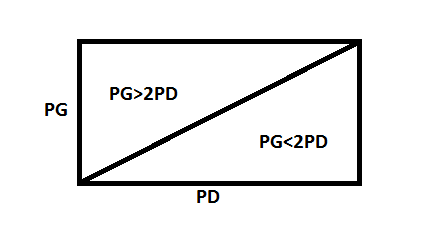
\includegraphics[scale=1]{q6}
        \caption{PG vs. PD}
\end{figure}



\end{document}